% vim: ft=tex
\chapter{Scope}
The technical goals of this bachelor thesis include extending mindclue GmbH's
Roadster framework by adding features such as clustering, high availability and
transport security. This chapter outlines the general scope of this project.

\section{Motivation}
% TODO Why do we care about this thesis? Why are we interested?\\

\subsection*{Backgrounds}
To better understand our motivation, it might help to understand our personal backgrounds first.

\begin{description}
	\item [Patrik Wenger]\hfill\\
		Having done his apprenticeship in computer science at Swisscom
		Schweiz AG, he continued to work as a full-time employee for
		five years afterwards. In programming he's most fluent in
		\gls{ruby} and \gls{c}. During the winter of 2015/2016, he
		created \gls{cztop} during leisure time because there was no
		good Ruby binding for \gls{zmq}/\gls{czmq} available and a side
		project of his demanded it.

		Fascinated with event-driven programming and software design
		patterns such as the \gls{actor-model}\footnote{known from
		Erlang, brought to Ruby by the Celluloid library, as well as the young
		programming language Pony which is completely based on actors},
		distributed computing and high availability have always been
		part of his core interests, especially in conjunction with the
		brilliant \zmq library.

		Having a passion for information security and state-of-the-art
		cryptography\footnote{such as \gls{nacl} or \gls{libsodium} as
		used by \gls{zmq}}, especially in this post-Snowden era, this
		bachelor thesis is like a dream come true.

	\item [Manuel Schuler]\hfill\\
		%TODO: Manuel: Javascript, .NET, horizont extension, learning new things, no hesitation for this project\\
		Always keen on learning new things, he did not hesitate to join
		this bachelor thesis at the first opportunity.
\end{description}

\noindent
In essence, we're both thrilled to gain more experience in the following
fields and technologies:

\begin{itemize}
	\item Distributed Computing
	\item High Availability
	\item Information Security
	\item \gls{actor-model}
	\item \gls{zmq}
	\item \gls{ruby}
\end{itemize}

\subsection*{Opportunities}
Coming from different backgrounds and having different levels of experience in
each of the above technologies, we can't wait to learn more about them and put
them to actual use. The fact that the product of this bachelor thesis is most
likely going to be used in the real world only adds to the excitement.

This bachelor thesis involves working with Ruby, the Actor Model, \zmq,
distributed computing with high availability, and state-of-the-art
cryptography. Furthermore, Roadster is a next-generation SCADA framework, and
the results of this thesis will be used in real-world settings like the Ceneri
Base Tunnel. It is a huge opportunity for a solution completely based on free
and open-source software. The students, as well as the client, strongly believe
in customized solutions built on reusable, free open-source software.

In addition to that, we look at this bachelor thesis as an opportunity to
become more fluent in English, both written and spoken, as well as to improve
our skills in crafting scientific documents using {\LaTeX}.

Depending on how we perform together as a team, further collaboration might
result in the future, either between the students themselves, or between the
students and the client. Even if our paths will part, this project will
serve as a valuable reference for future job hunting.

Last but not least, we feel like Prof. Dr. Mehta is a respected and competent
teacher whose opinions we highly value. Due to his polite parlance, discussing
project matters, both of the management and the technical kind, has always been
an enrichment.

\subsection{Open-Source Engagement}
TODO spread of CZTop and proof of its design\\
TODO creation of cztop-patterns (as mentioned in the Mgmt Summary)\\

\section{Initial Situation}

\subsection{mindclue GmbH}
\subsubsection{About}
The company mindclue GmbH, located in Ziegelbr\"ucke provides its partner
REMTEC AG with complete SCADA applications. These are then used to control and
monitor operational and safety equipment found in national freeways, water
supply systems, as well as in energy facilities and many other specialized
fields. To build these customized applications, their in-house creation
Roadster, a next-generation SCADA framework, is used.

\subsubsection{Roadster}
Roadster ist eine Ereignis gesteuerte Applikation geschrieben in Ruby.
Sie ist die eigentliche \gls{SCADA} Applikation und wird bereits in einer Vielzahl von
Tunnelanlagen in der Schweiz eingesetzt und dient zur Überwachung der einzelnen Komponenten im Tunnel.
Durch den modularen Aufbau kann jede Roadster Applikation sich selbst laufen - Autonom.
Sprich jeder Roadster hat seinen eigenen Webserver und Datenverwaltung.

\subsubsection{AS - UeLS}
Roadster ist einer von vielen AS Knoten eines UeLS. Die Kommunikation
zwischen AS und AR geschieht über "OPC UA".
%TODO .... include graphics as_detail and overall system


\subsection{\zmq}
\emph{For a more detailed introduction, see \autoref{ch:zmq}.}

To understand Roadster's architecture and the rest of this document, it's
helpful to understand the basics of \zmq (sometimes written as ZeroMQ or simply
ZMQ) first. This is a brief introduction to \zmq for the unfamiliar reader.

\zmq is a \gls{MOM} implemented as an open source library, that is, it doesn't
require a dedicated broker. Instead, it offers sockets with an abstract
interface similar to \acrshort{BSD} sockets. Different types of sockets are used for
different messaging patterns such as request-reply, publish-subscribe, and
push-pull.

A single socket can bind/connect to multiple endpoints, which allows \zmq to
use round-robbin on the sender side, and fair-queueing on the receiver side,
where applicable. It doesn't matter whether the communication happens
in-process (between threads), inter-process (e.g. over \glspl{unix-domain-socket}), or
inter-node (e.g. over \acrshort{TCP}/\acrshort{PGM}/\acrshort{TIPC}), since the transport is completely
abstracted away. The same goes for connection handling; an arbitrary amount of
connections is handled over a single socket and reconnecting after short
network failures is done transparently.

\zmq is lightweight and provides extremely low latencies, which means it can
also be used as the fabric of concurrent applications, e.g. for the actor
model. In case of the TCP transport, it incorporates advanced techniques such
as smart message batching to achieve significantly higher throughputs than with
raw TCP or other \gls{MOM} solutions \cite[Figure 2, Middleware evaluation and
prototyping, p.~4]{cern:new-cmw}.

To build a solution with \zmq, its sockets are used as building blocks to
design custom message flows. Certain patterns are used to achieve reliability
with respect to the failure types that need to be addressed in particular.  The
zguide\footnote{\url{http://zguide.zeromq.org/}} explains best practices,
including commonly needed, resilient messaging patterns.

The above characteristics make \zmq a valuable asset when it comes to building
robust, distributed high-performance systems.

\subsubsection{Transport Security}
Since version 4.0, \zmq boasts state of the art encryption and authentication,
based on the excellent and highly renown
\gls{nacl}\footnote{\url{http://nacl.cr.yp.to}} library.

\subsubsection{Data Serialization}
Data serialization is outside the scope of \zmq. To fill the gap, one typically
uses another library such as MsgPack\footnote{\url{http://msgpack.org}},
Protocol
Buffers\footnote{\url{https://developers.google.com/protocol-buffers/}}, or
even a programming language's built-in object serialization
support\footnote{such as Ruby's marshalling support:
\url{http://ruby-doc.org/core/Marshal.html}}.

\subsubsection{CZMQ}
\gls{czmq} is a high-level abstraction layer for \zmq. It makes working with the \zmq
library more expressive and allows for better portability. It also provides
additional functionality such as a reactor, a simple actor implementation, as
well as utilities for certificate and authentication handling, and LAN node
discovery. This is the recommended way of using \zmq nowadays.

\subsection{Software Architecture}
TODO more\\

Roadster is event-driven and built on the Actor model, meaning it exhibits a
shared-nothing architecture. Each Roadster node runs a number of Ruby processes
which communicate via \zmq sockets. The key here is communication:

\begin{quote}
``Don't communicate by sharing state; share state by communicating.''
\end{quote}

Running multiple, loosely coupled processes (actors) allows leveraging the full
potential of modern multi-core processors, while avoiding a whole class of
traditional concurrency problems.

Every Roadster node runs a group of actors:

\begin{description}
	\item [CORE:]
		It is responsible to start the other actors. It also plays a
		key role in keeping state in all actors synchronized, being the
		source of truth.

	\item [COMM:]
		A bunch of COMM actors communicate with the outside world of a
		node. This can be different kind of \glspl{PLC} or higher level
		monitoring systems. Each COMM actor uses an adapter
		specifically written for a single communication protocol.

	\item [STORAGE:]
		This actor is used when information needs to be persisted, such
		as time series or event journals. It's the interface to a
		key-value store.

	\item [LOGGER:]
		This actor collects logging data and sends it to whatever
		target is configured, be it STDOUT, a file, or a syslog server.
\end{description}

\autoref{fig:roadster:arch} illustrates Roadster's architecture.

\begin{figure}[!ht]
	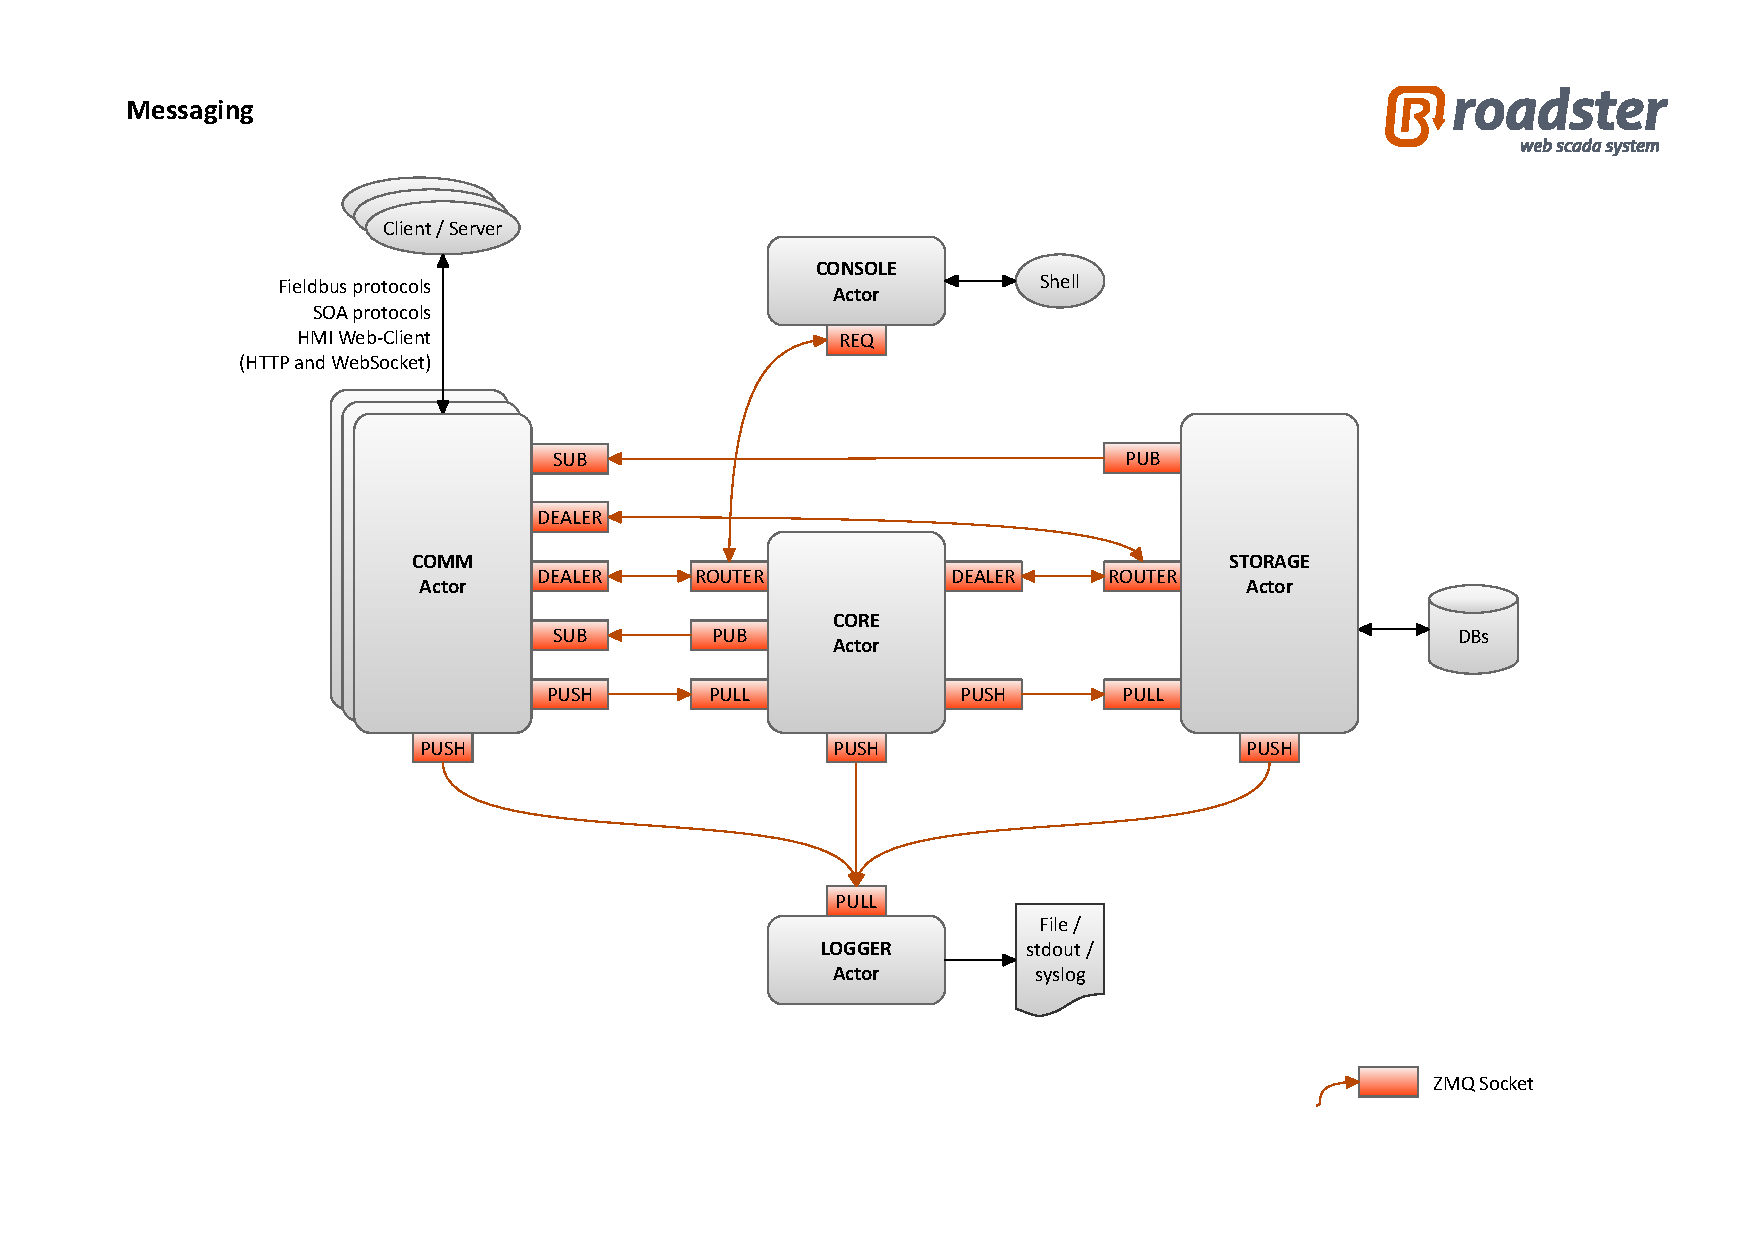
\includegraphics[trim=4cm 2cm 3.5cm 2.8cm, clip=true, width=\textwidth]{img/roadster_arch.pdf}
	\source{Andy Rohr}
	\caption{Roadster's software architecture}
	\label{fig:roadster:arch}
\end{figure}

\subsubsection{Communication Layers}
The communication architecture in Roadster consists of three layers, as
illustrated in \autoref{fig:roadster:layers}. The following list briefly
explains the layers from top (most abstracted) to bottom:

\begin{description}
	\item [Engine layer:]\hfill\\
		Here is the business logic of Roadster, e.g. the \gls{DIM},
		user authentication, adapters for different devices, the web
		\gls{UI}, etc.

	\item [Messaging layer:]\hfill\\
		The \gls{RMP} reside here implement essential protocols used
		for logging, state synchronization, commands, application
		shutdown, and storage. They're explained below.

	\item [Reactor layer:]\hfill\\
		This layer forms the base, which is where the \zmq sockets and
		WebSockets used. In case of COMM actors, there can also be raw
		TCP sockets, e.g. to interact with certain \glspl{PLC}.
\end{description}

\begin{figure}[!ht]
	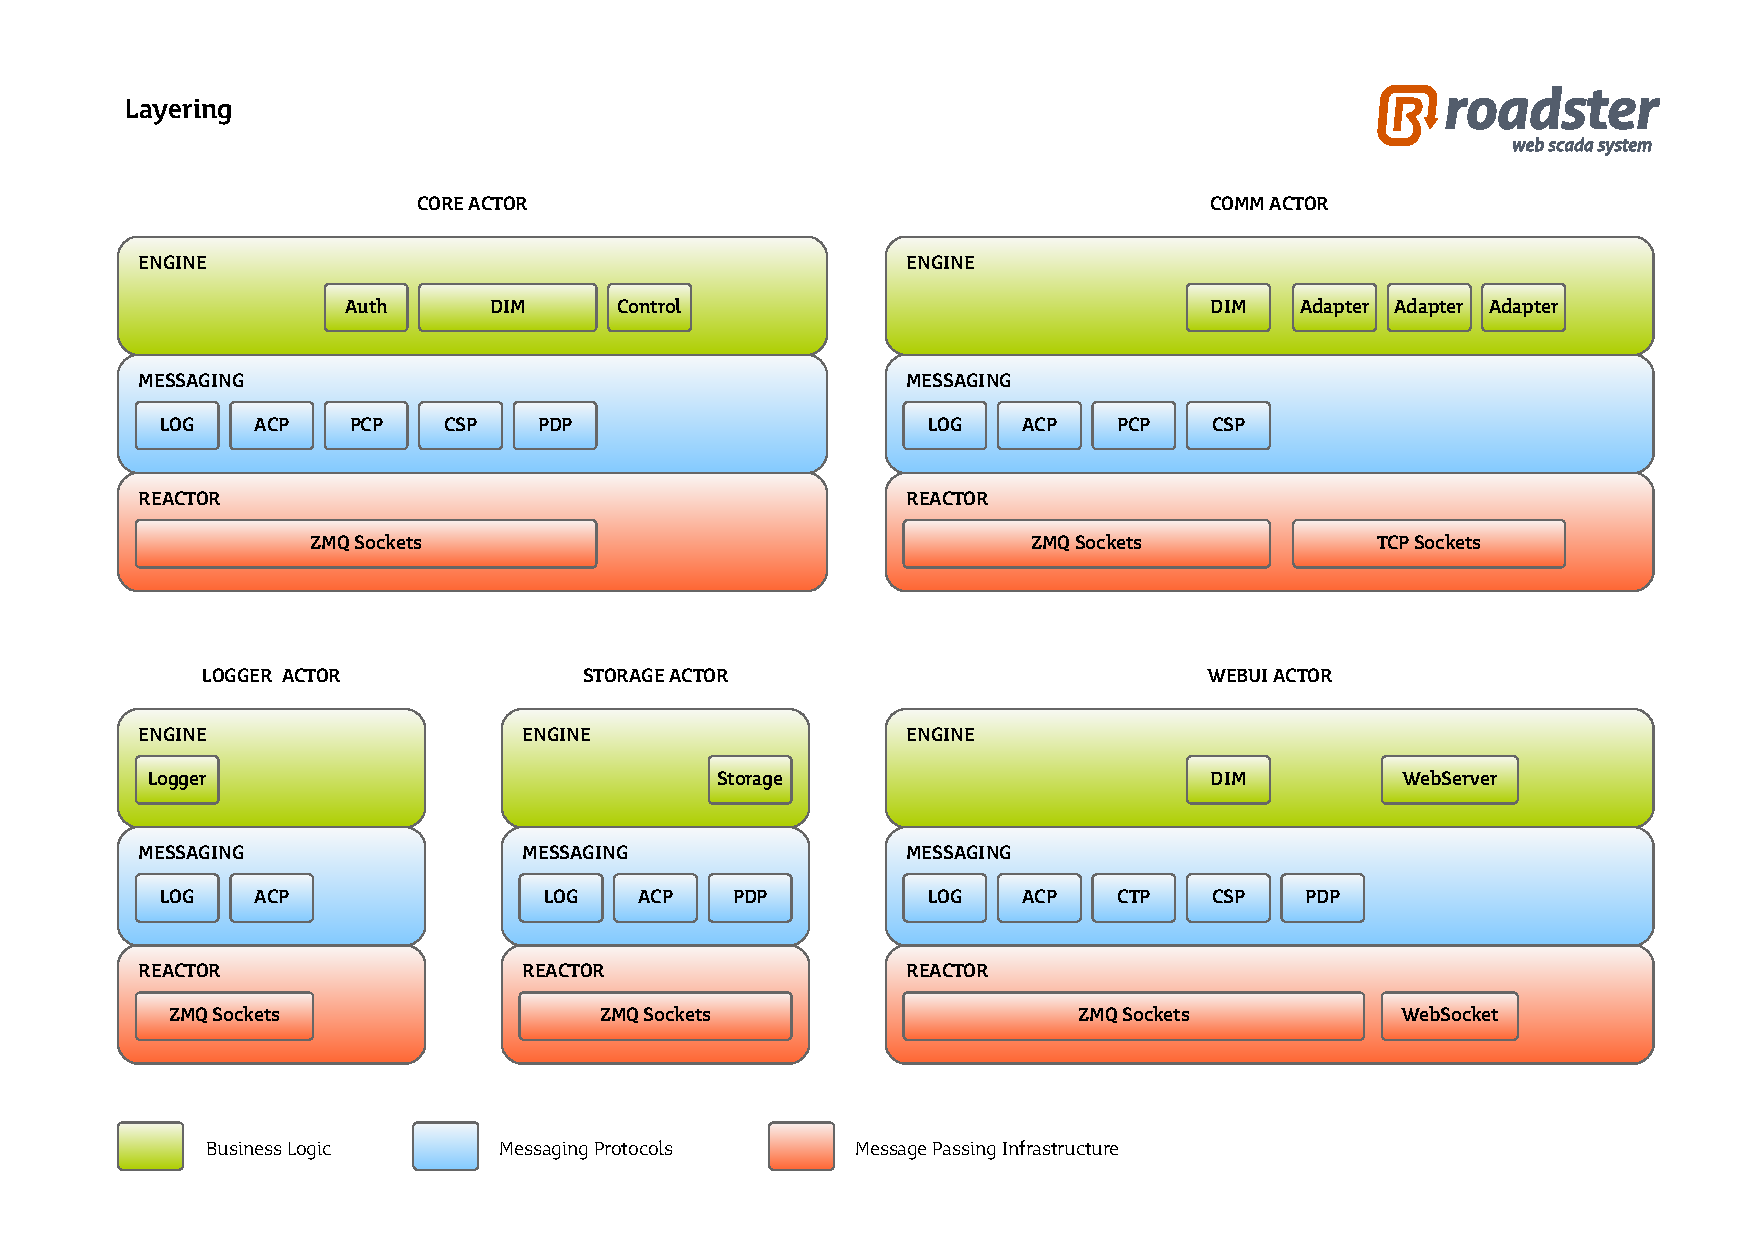
\includegraphics[trim=1.95cm 2.5cm 1.65cm 2.8cm, clip=true, width=\textwidth]{img/roadster_layering.pdf}
	\source{Andy Rohr}
	\caption{Roadster's communication layers}
	\label{fig:roadster:layers}
\end{figure}

\subsubsection{RMP}
The \gls{RMP} are a collection of protocols implemented and used by Roadster
internally. They reside in the messaging communication layer, and include:

\begin{description}
	\item [\gls{CSP}:]\hfill\\
		Used to synchronize state between the actors.
	\item [\gls{ACP}:]\hfill\\
		Used to control the application state, e.g. things like shutdown.
	\item [\gls{PDP}:]\hfill\\
		Used when data needs to be persisted.
	\item [\gls{SMP}:]\hfill\\
		Used to suppress the generation of certain \glspl{case}, e.g.
		when a sensor is defect and repeatedly causes cases.
	\item [\gls{CTP}:]\hfill\\
		Used for asynchronous command execution with feedback.
	\item [\gls{LOG}:]\hfill\\
		Used for system logging.
\end{description}

Every actor in Roadster uses a subset of these protocols to perform its job.

% Fire+Forget: no guarantee of correct processing. E.g. DIM updates from COMM to CORE
% TODO: Dialogs: immediate answer, synchronous looking code (but still handled with async messaging). E.g. creating a user session

\section{Goals}
TODO preprocessed mandatory goals\\
TODO retrospective, diff with initial goals\\

To summarize the goals from the Task Description in \autoref{ch:task-desc}:

\begin{enumerate}
	\item Extending communication protocols to support clustering
	\item Extending communication protocols to add high availability
\end{enumerate}

An implication of the above goals is secure inter-node communication in a Roadster cluster. This is also to mitigate common security concerns with SCADA systems which are becoming more and more open due to standardization. To quote wikipedia:

TODO move this part somewhere else, a section dedicated to security in SCADA systems
\begin{quote}

``In particular, security researchers are concerned about:
	\begin{itemize}
		\item the lack of concern about security and authentication in the design, deployment and operation of some existing SCADA networks
		\item the belief that SCADA systems have the benefit of security through obscurity through the use of specialized protocols and proprietary interfaces
		\item the belief that SCADA networks are secure because they are physically secured
		\item the belief that SCADA networks are secure because they are disconnected from the Internet.''
	\end{itemize}
\end{quote}

\subsection*{Optional Goals}
TODO optional goals

\begin{enumerate}
	\item Encryption of the communication
	\item Providing of the highly available \gls{OPC} \gls{UA} server interface
\end{enumerate}


TODO The Eight Fallacies of Distributed Computing
https://blogs.oracle.com/jag/resource/Fallacies.html
